\documentclass[11pt]{article}
\usepackage[super,square,comma]{natbib}
\usepackage[letterpaper, margin=1.25in]{geometry}
\usepackage{tikz}
\usepackage{lipsum}
\usepackage{setspace}
\usepackage{enumerate}
\usepackage[inline, shortlabels]{enumitem}
\usepackage{amsmath}
\newtheorem{problem}{Problem}
\numberwithin{equation}{section}

\usepackage{listings}

\newcommand\pythonstyle{\lstset{
language=Python,
basicstyle=\ttm,
otherkeywords={self},             % Add keywords here
keywordstyle=\ttb\color{deepblue},
emph={MyClass,__init__},          % Custom highlighting
emphstyle=\ttb\color{deepred},    % Custom highlighting style
stringstyle=\color{deepgreen},
frame=tb,                         % Any extra options here
showstringspaces=false            % 
}}


\usepackage{animate}
\usepackage{siunitx}
\usepackage{csquotes}
\usepackage{graphicx}
\usepackage{authblk}
\usepackage[labelfont=bf]{caption}
\usepackage{subcaption}

\usepackage{fancyhdr}
\pagestyle{fancy}
\lhead{Team 93463}
\chead{\textsc{Multi-hop, HF Radio Propagation Near Japan}}
\rhead{Page \thepage\ of \pageref{LastPage}}
\setlength{\headheight}{14pt}

\usepackage{lastpage}

\renewcommand{\thefootnote}{\arabic{footnote}}
\newcommand{\cn}{$^{\text{[citation needed]}}$} %citation needed

% %%% Title Page Author Stuff %%%
% \renewcommand*{\Authsep}{, }
% \renewcommand*{\Authand}{, }
% \renewcommand*{\Authands}{, }
% \renewcommand*{\Affilfont}{\normalsize\normalfont}
% % \renewcommand*{\Authfont}{\bfseries}    % make author names boldface    
% \setlength{\affilsep}{1em}   % set the space between author and affiliation

% \newsavebox\affbox

% \author[1]{Colin M. Adams}
% \author[1]{Rachel L. Barcklay}
% \author[1,2]{Carla J. Becker}
% \affil[1]{%
%   \savebox\affbox{\Affilfont Department of Physics, Harvey Mudd College}%
%   \parbox[t]{\wd\affbox}{\protect\centering Department of Physics, Harvey Mudd College}} 
% \affil[2]{Department of Chemistry, Harvey Mudd College \par Claremont, CA 91711}


%%%%%%%%%%%%%%%%%%%%%%%
\renewcommand{\baselinestretch}{2}
\newcommand{\shrug}[1][]{%
\begin{tikzpicture}[baseline,x=0.8\ht\strutbox,y=0.8\ht\strutbox,line width=0.125ex,#1]
\def\arm{(-2.5,0.95) to (-2,0.95) (-1.9,1) to (-1.5,0) (-1.35,0) to (-0.8,0)};
\draw \arm;
\draw[xscale=-1] \arm;
\def\headpart{(0.6,0) arc[start angle=-40, end angle=40,x radius=0.6,y radius=0.8]};
\draw \headpart;
\draw[xscale=-1] \headpart;
\def\eye{(-0.075,0.15) .. controls (0.02,0) .. (0.075,-0.15)};
\draw[shift={(-0.3,0.8)}] \eye;
\draw[shift={(0,0.85)}] \eye;
% draw mouth
\draw (-0.1,0.2) to [out=15,in=-100] (0.4,0.95); 
\end{tikzpicture}}


\title{
    \textsc{{Multi-hop, High-Frequency Radio Propagation Near Japan}}
    }

\author{\Large Team 93463}
\date{\today}
        

\begin{document}
%%%%%%%%%%%%%%%%%%%%%%%%%%%%%%%%%%%%%%%%%%%%%%%%%%%%%%%%%%%%%%%%%%%%%%
% Title Page
%%%%%%%%%%%%%%%%%%%%%%%%%%%%%%%%%%%%%%%%%%%%%%%%%%%%%%%%%%%%%%%%%%%%%%
    \singlespacing %sets spacing of abstract to single
    \clearpage
    \maketitle
    \thispagestyle{empty} %gets rid of page number at bottom 

    \begin{center}
        \rule{13cm}{0.4pt}  
    \end{center}

    \noindent To whom it may concern, \vspace{4pt}\\
    %
    \indent When reading our solution, we hope that you are can read it using Adobe Acrobat Reader. This is because we have \texttt{.gif} files that can only be played with that particular PDF reader. Please visit \texttt{https://get.adobe.com/reader/} to download it if necessary. We are trying to put our best foot forward and we would appreciate if you receive our work as intended. We believe it is worth it. Thank you.
    \vspace{4pt} \\ 
    Respectfully,\vspace{3pt}\\
    \indent Team 93463
    \begin{center}
        \rule{13cm}{0.4pt}  
    \end{center}

\newpage

%%%%%%%%%%%%%%%%%%%%%%%%%%%%%%%%%%%%%%%%%%%%%%%%%%%%%%%%%%%%%%%%%%%%%
%% Body
%%%%%%%%%%%%%%%%%%%%%%%%%%%%%%%%%%%%%%%%%%%%%%%%%%%%%%%%%%%%%%%%%%%%%
\setcounter{page}{1} %set new page number to 1

\section{Motivation} % (fold)
\label{sec:motivation}

Quickly after its invention in the late 19th century, radio was adopted worldwide as the main form of communication for long distances near instantaneously.\cite{hilmes2002radio} When utilized correctly, the radio has accomplished remarkable things. Radios have inspired generations of scientists and tinkerers; they have allowed world-leaders to communicate with their people, soldiers to their brothers-in-arms,\footnote{Yes, we know. This terminology is a little dated.} they have allowed music to spread across cultures, and they have allowed Alex Jones spout gibberish to conspiracy theorists across the United States.\footnote{Enjoy. \texttt{https://youtu.be/aCiVsJ3b160}} 

However, the often catastrophic failures of radio have been a result of not understanding the science behind them. For example, a poor understanding of the Titanic's radio contributed to the deaths of 1,514 passengers and crew from April 14--15, 1912.\cite{noauthor_radio_2011} While much---if not most---of the engineering difficulties of radio have been overcome, some of the fundamental science behind it has not, e.g. ground-wave propagation.\cite{budden1961radio} To avoid other horrendous accidents at sea, such as the Titanic, it's important to have an accurate model of how radio-waves propagate through the atmosphere to determine the maximum distance a signal can travel at sea.

Our task, if we choose to accept it,\footnote{Cue the \emph{Mission Impossible} theme song: Dun Dun Dun da dada Dun dun dun da dada dun dun dun da dada, de da doo de da doo de da doo do dut.} is to solve the following three problems:
\begin{problem}
 The first problem we are trying to solve is to determine how many times a HF radio-wave can be reflected off of the ocean. The first reflection of the signal is off of a turbulent ocean. We must characterize how the signal strength changes after this first reflection. After the first reflection, we are looking to characterize how the signal changes as it reflects off of calm oceans before falling below a signal to noise ratio (SNR) of 10\,\si{\dB}.
 \label{pr:turb_ocean}
\end{problem}

\begin{problem}
    This is the same problem as Problem \ref{pr:turb_ocean}, but instead of the ocean, we have rugged and smooth terrain.
    \label{pr:mount}
\end{problem}

\begin{problem}
    Lastly, we would like to see how a boat traveling across the ocean using HF radio-waves to communicate and how our model changes to accommodate a receiver in motion on a turbulent ocean.
    \label{pr:boat}
\end{problem}
% section motivation (end)

\section{Introduction} 
\label{sec: intro} 

 \begin{figure}[ht]
 \begin{center}
     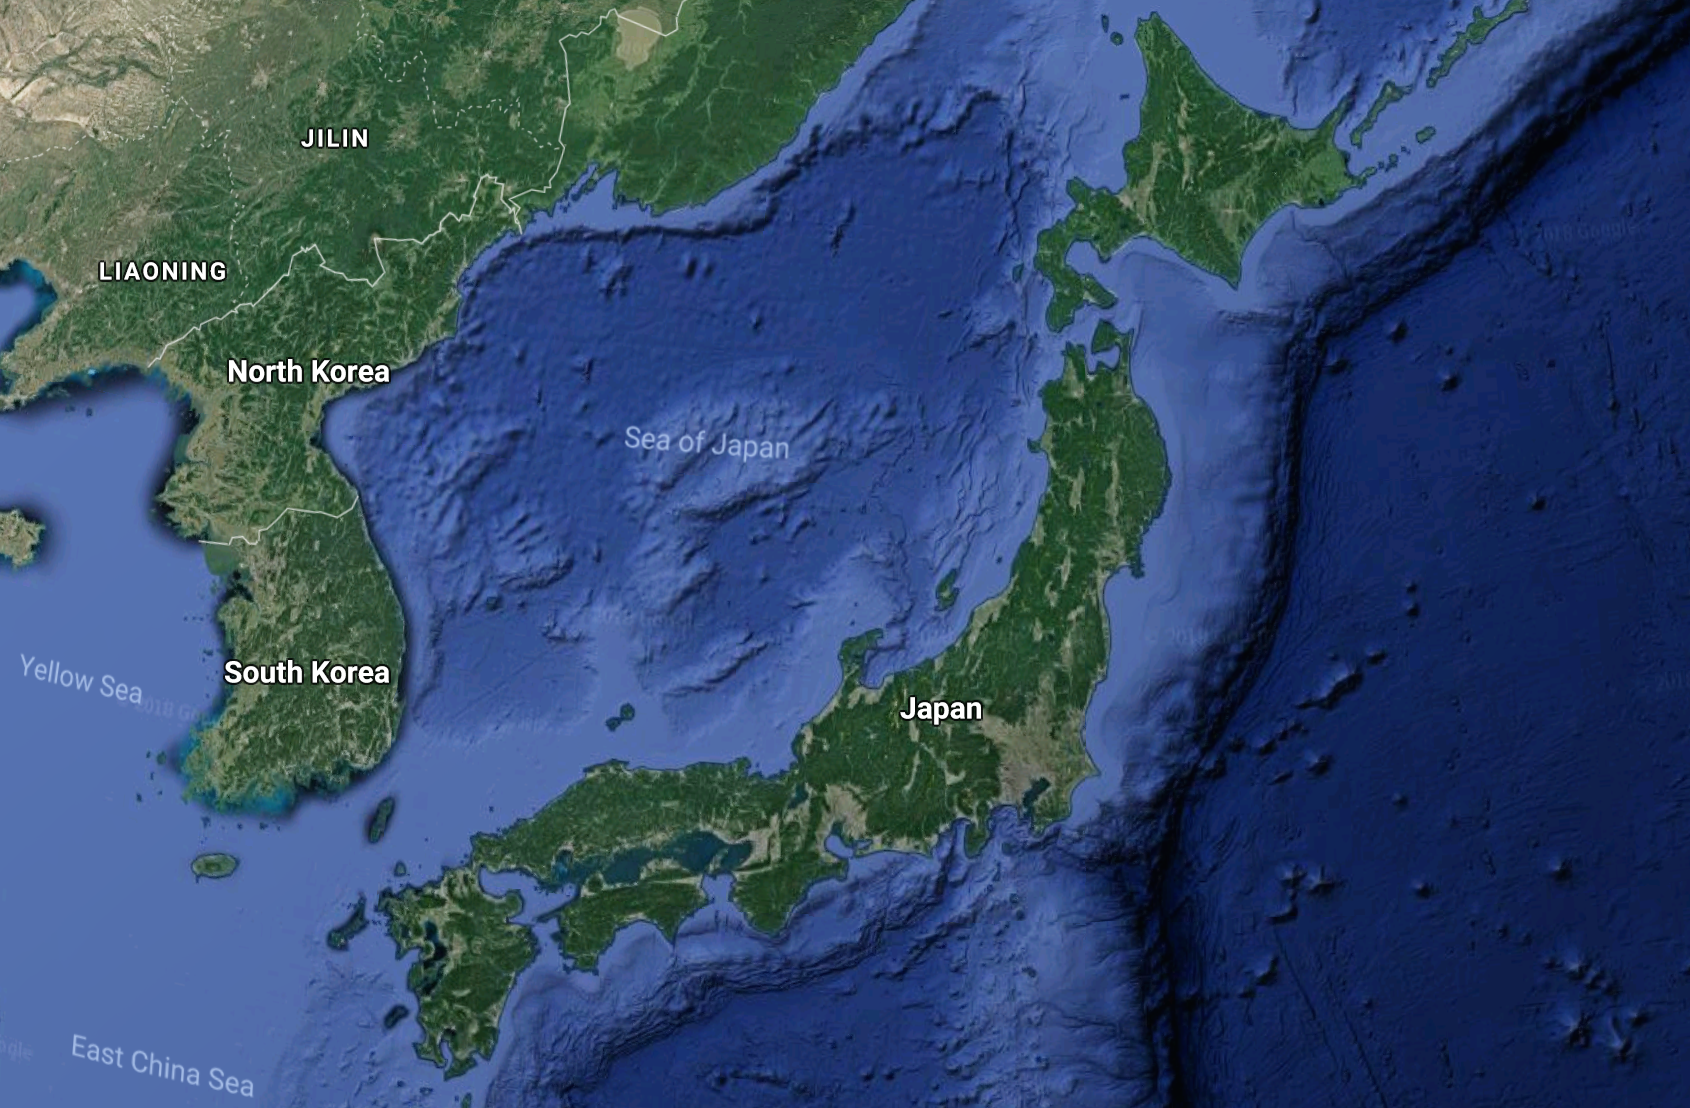
\includegraphics[width = 4.55in]{figs/japan.png}
 \end{center}
 \caption{The region we are studying. Japan was chosen due to it being a very mountainous and rugged island surrounded by ocean water. Image taken from Google Maps.}
 \label{fig:jap} 
\end{figure} 

High frequency radio-waves (defined to be between 3--30\,\si{\mega\hertz}) can travel through the atmosphere---by one mechanism---by multiple reflections off of the Earth's ionosphere and the its surface. For frequencies below the maximum usable frequency (MUF), they will skip from the surface of the earth to the ionosphere and back again indefinitely until the signal dies down and becomes unusable. If the frequencies are larger than the MUF, then they pass through the ionosphere and are lost to space forever. The MUF varies with the season, time of day, and solar conditions.\cite{mcm_statement} In our model, we will neglect solar conditions for simplicity.


Empirically, radio-waves reflect off of the ocean differently depending on whether the ocean is turbulent or calm, impacting the distance the signal can faithfully.\cite{mcm_statement} Not surprisingly, radio-waves will reflect off rugged terrain differently than smooth, making it important to model how these radio-waves travel over mountains as well.

With this in mind, we decided to focus on a region of with a radius of roughly 550\,\si{\km} from Tokyo, Japan (Fig.\ref{fig:jap}). We chose this location because there is a large quantity of reliable data taken in Japan, it is an island country, and is ``mostly rugged and mountainous.''\cite{factbook2010world} In essence, it is an ideal location to accurately study high-frequency (HF) radio-waves and their interactions with ionosphere and ocean.


\section{Model} % (fold)
\label{sec:model}

To have an accurate model, there are three main components of this model that need to be described. Primarily, we need to be able to describe HF radio-waves and how they change with reflections and gather inherent noise when travelling through a medium. Because our signal reflects off of two different interfaces as it travels---the ocean and the ionosphere---it is important to model each with accurate physical properties. We would like to see how they change with time of day and time of year. 
\subsection{Radio-waves} % (fold)
\label{sub:radiowaves}

\subsubsection{Underlying Electromagnetic Theory} % (fold)
\label{ssub:emtheory}

Any rightful modeling of radio waves begins with Maxwell's Equations. For our purposes, we will only model the electric field component of the radio waves and we will consider a two-dimensional problem wherein the reflected and transmitted waves are in the plane of incidence. Let this electric field component of a single Fourier component of the incident radio wave be given by
\begin{equation}
{\bf \tilde{E}}_{I}({\bf r}, t) = {\bf \tilde{E}}_{0_I} e^{i({\bf k}_{I} \cdot {\bf r} - \omega t)}
\end{equation}
where ${\bf \tilde{E}}_{0_I}$ is the complex magnitude of the component, $\theta_{I}$ is the angle of incidence to the surface (which will eventually be either ocean or ionosphere), ${\bf k}_{I}$ is the wave vector of the incident component, and $\omega$ is the frequency characterizing this Fourier component.
\par We then also consider the Law of Reflection (\ref{eq:refl}) and Law of Refraction (\ref{eq:refr}):
\begin{equation}
\theta_{I} = \theta_{R}
\label{eq:refl}
\end{equation}
\begin{equation}
\frac{\sin\theta_{T}}{\sin\theta_{I}} = \frac{n_1}{n_2}
\label{eq:refr}
\end{equation}
where the subscripts $R$ and $T$ refer to reflection and transmission respectively. Using Fresnel's equations \ref{eq:fresnel} for light polarized horizontal to Earth's surface (as this polarization can reach larger distances with less attenuation)
\begin{equation}
\tilde{E}_{0_R} = \left( \frac{\alpha - \beta}{\alpha + \beta} \right)\tilde{E}_{0_I}, \qquad 
\tilde{E}_{0_T} = \left( \frac{2}{\alpha + \beta} \right)\tilde{E}_{0_I}
\label{eq:fresnel}
\end{equation}
along with the angle of incidence $alpha$, average altitude of the ionosphere $h$, height of the transmission tower $z$, index of refraction of the ionosphere and ocean (as a function of incident frequency, time of day, time of year, and roughness of sea), and dielectric constant of air, we can calculate how the signal is attenuated in frequency space. In \ref{eq:fresnel}, $\alpha$ and $\beta$ are given by
\begin{equation}
\alpha = \frac{\cos\theta_{T}}{\cos\theta_{I}}, \qquad \beta \approx \frac{n_1}{n_2}
\end{equation}
where we have made the approximation that the permeability of all materials involved is approximately the vacuum permeability, which is a solid assumption for most materials.\cite{griffiths2005introduction} 
\par We also assume that both the ocean and ionosphere are conducting, linear, dispersive media such that a wave reflected has its amplitude attenuated by the term
\[
e^{-\kappa z}
\]
where $\kappa$, derived from Maxwell's equations for linear, conducting media\cite{griffiths2005introduction}, is given by
\begin{equation}
\kappa = \omega \sqrt{\frac{\epsilon\mu}{2}}\left[ \sqrt{1 + \left( \frac{\sigma}{\epsilon\omega} \right)^2} - 1 \right]^{1/2}
\end{equation}
where $\sigma$ is the electrical conductivity of air, $\epsilon$ is the permittivity of air, and $\mu$ is the permeability of air.
\par For a full listing of constants used throughout our modeling, see the Appendix and the file \verb|constants.py|.

 \begin{figure}
     \begin{center}
        \animategraphics[width=4.25in]{12}{gif/frame-}{0}{99}
     \end{center}
     \caption{ Click image to see animation. (You need to use Adobe Acrobat Reader to view this \texttt{.gif} file. If you do not have it, please visit \texttt{https://get.adobe.com/reader/} to download it. It is worth it.)}
 \end{figure}
 
As an introduction to the results of our modeling, we have produced an animation of signal decay over the first 30 seconds as it propagates toward Los Angeles from Tokyo, with incident angle 30 degrees above parallel to Earth's surface. Over that distance, the signal reflects off of the ionosphere and ocean 8 times each. The signal above has two Fourier components and is not a simple carrier wave. The animation represents signal propagation under ``nice" weather conditions. The addition of noise, though accounted for in our model, is not shown in the animation. 

\subsubsection{Noise} % (fold)
\label{ssub:noise}

As radio-waves propagate over a certain distance, we expect them to pick up some noise as they go, degrading the integrity of the information they are trying to transmit. If they didn't, you could presumably use a \$5 hand-held radio to communicate with police officers in Australia.\footnote{It doesn't. One of the authors tried as a child.} A reasonable question becomes, how should we try and model this.

The Central Limit Theorem states that when using independent, random variables\footnote{We are assuming this in our model.} are added together, their properly normalized sums tend toward a normal distribution.\cite{central} So as the radio-wave travels, we add this Gaussian noise to the signal to degrade it as its path length increases. It turns out that this is used quite often in Information Theory, and is called Additive White Gaussian Noise (AWGN).\cite{shannon1984communication,kailath1968innovations}

\begin{figure}[ht]
 \begin{center}
     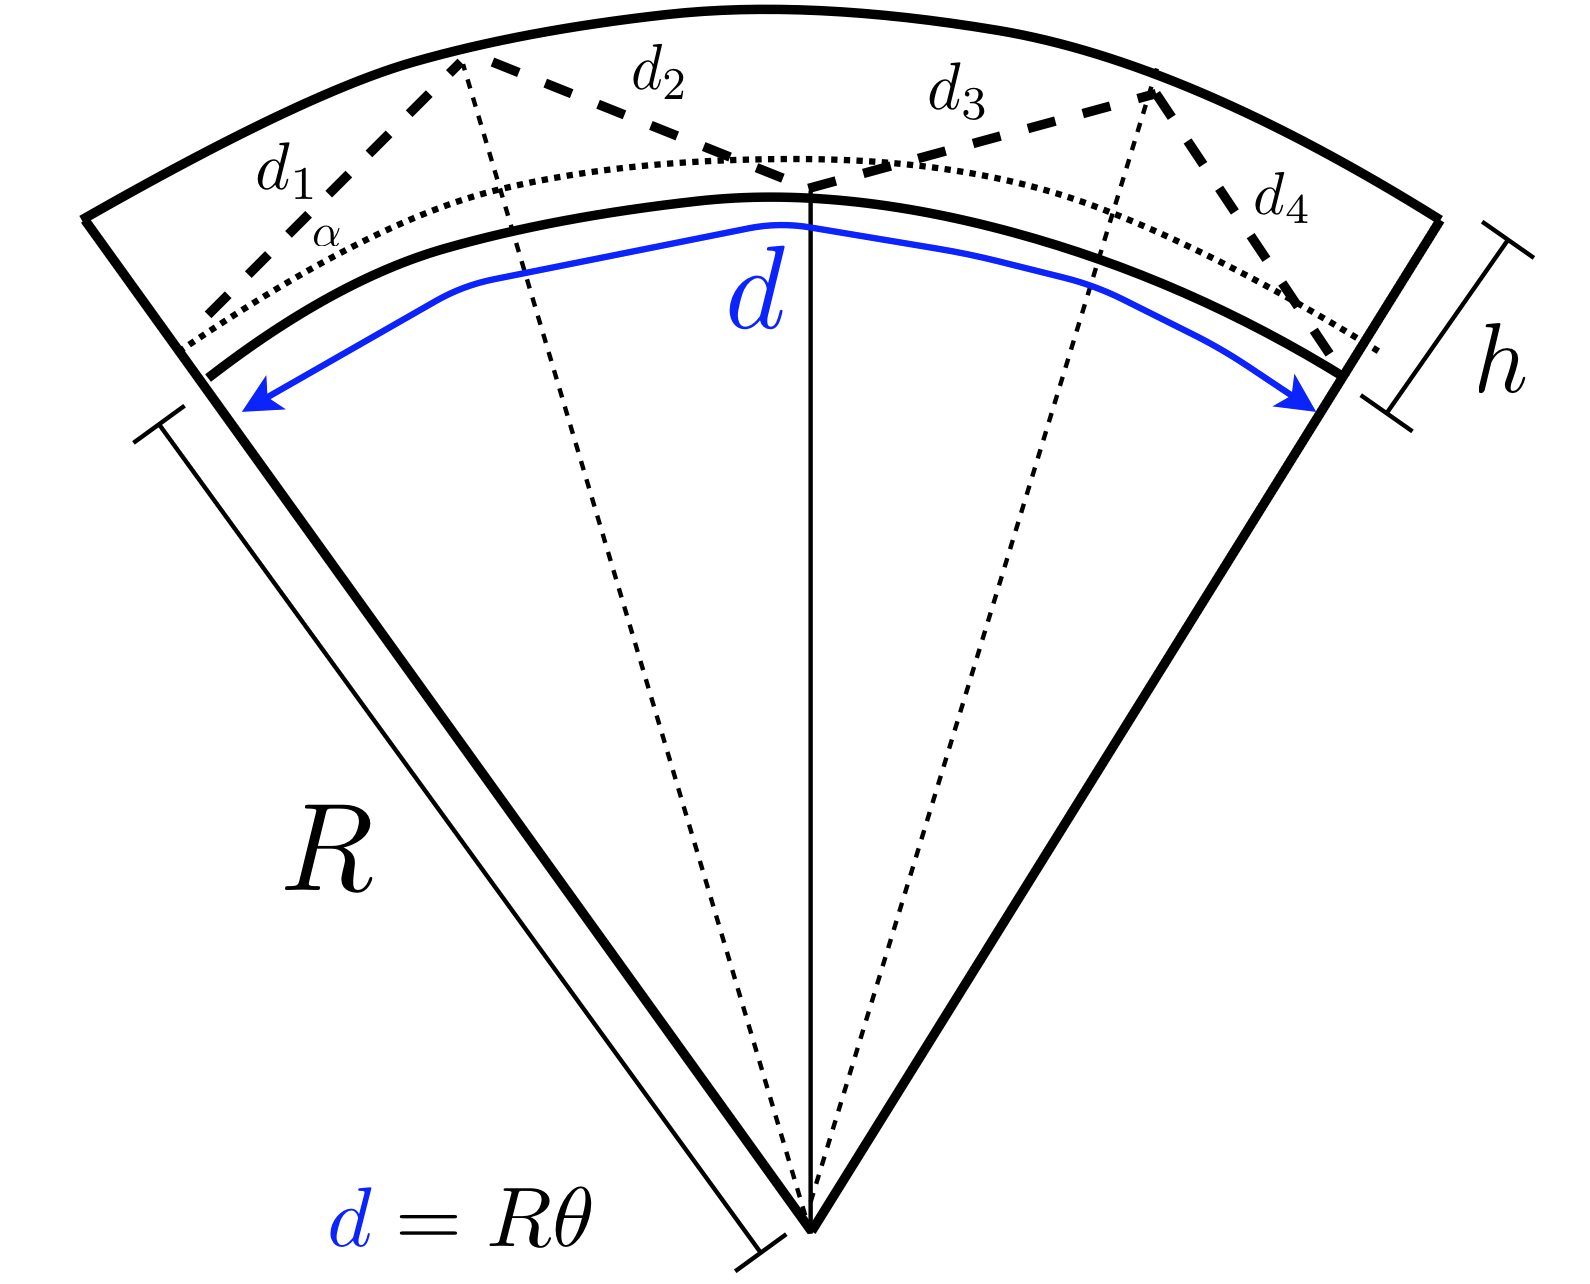
\includegraphics[width = 3.in]{figs/radio_curve.png}
 \end{center}
 \caption{A side diagram of how the HF signals travel through the atmosphere.}
 \label{fig:radio_curve}
\end{figure}

We modeled such that the standard deviation of this noise is proportional to the number of hops and the level of water turbulence, a decimal from 0-1 with 1 being the most turbulent.
% subsubsection noise (end)
% subsection radiowaves (end)

\subsection{The Ionosphere} % (fold)
\label{sub:the_ionosphere}

The ionosphere consists of roughly three layers that lie between 75--1000\,km above the Earth's surface:
\begin{enumerate*}[(1)]
    \item the F-region,
    \item the E-region, and
    \item the D-region
\end{enumerate*}; each of these regions has charge-density dependent on the time of year, the number of sunspots present, the time of day, and the movement of the charged particles\footnote{The study of which has the impressive sounding name of magnetohydrodynamics.}(Figure \ref{fig:struct_ion}). X-rays, ultraviolet light, ejected plasma, and other high energy particles that are released by the sun interact with the atoms in the atmosphere and strip them of electrons.\cite{noauthor_tracking_nodate} The ionosphere interacts heavily with radio waves, mainly through the interaction of these free electrons.\cite{budden1961radio}

Early experiments demonstrated that the electrons in the ionosphere are arranged in approximately horizontal layers, meaning that the number density is a function of height above the Earth's surface. Presumably, these cations are  atoms or molecules stripped of an electron. Because the ratio between the mass of a proton (the smallest positive charge we could have in the atmosphere) and an electron is on the order of $2\times10^3$, we would expect there must be approximately $5 \times10^{-4}$ more cations than electrons.\footnote{This is because the electric field of the propagating radio-waves will have $5 \times10^{-4}$ of the effect on a proton than an electron because its acceleration $\mathbf{a} \propto 1/m$.} If this were the case, the ionosphere would be unstable, due to the large repulsive forces of this unbalanced positive charge. However, due to the ionosphere's empirically determined and stable layers, the ionosphere must be nearly electrically neutral, i.e. there must be an equal number of positive and negative charges per unit volume.\cite{budden1961radio} Consequently, we assume that the radio-waves only interact with the free electrons in the ionosphere.

\begin{figure}[ht]
 \begin{center}
 \begin{subfigure}[b]{0.44\textwidth}
    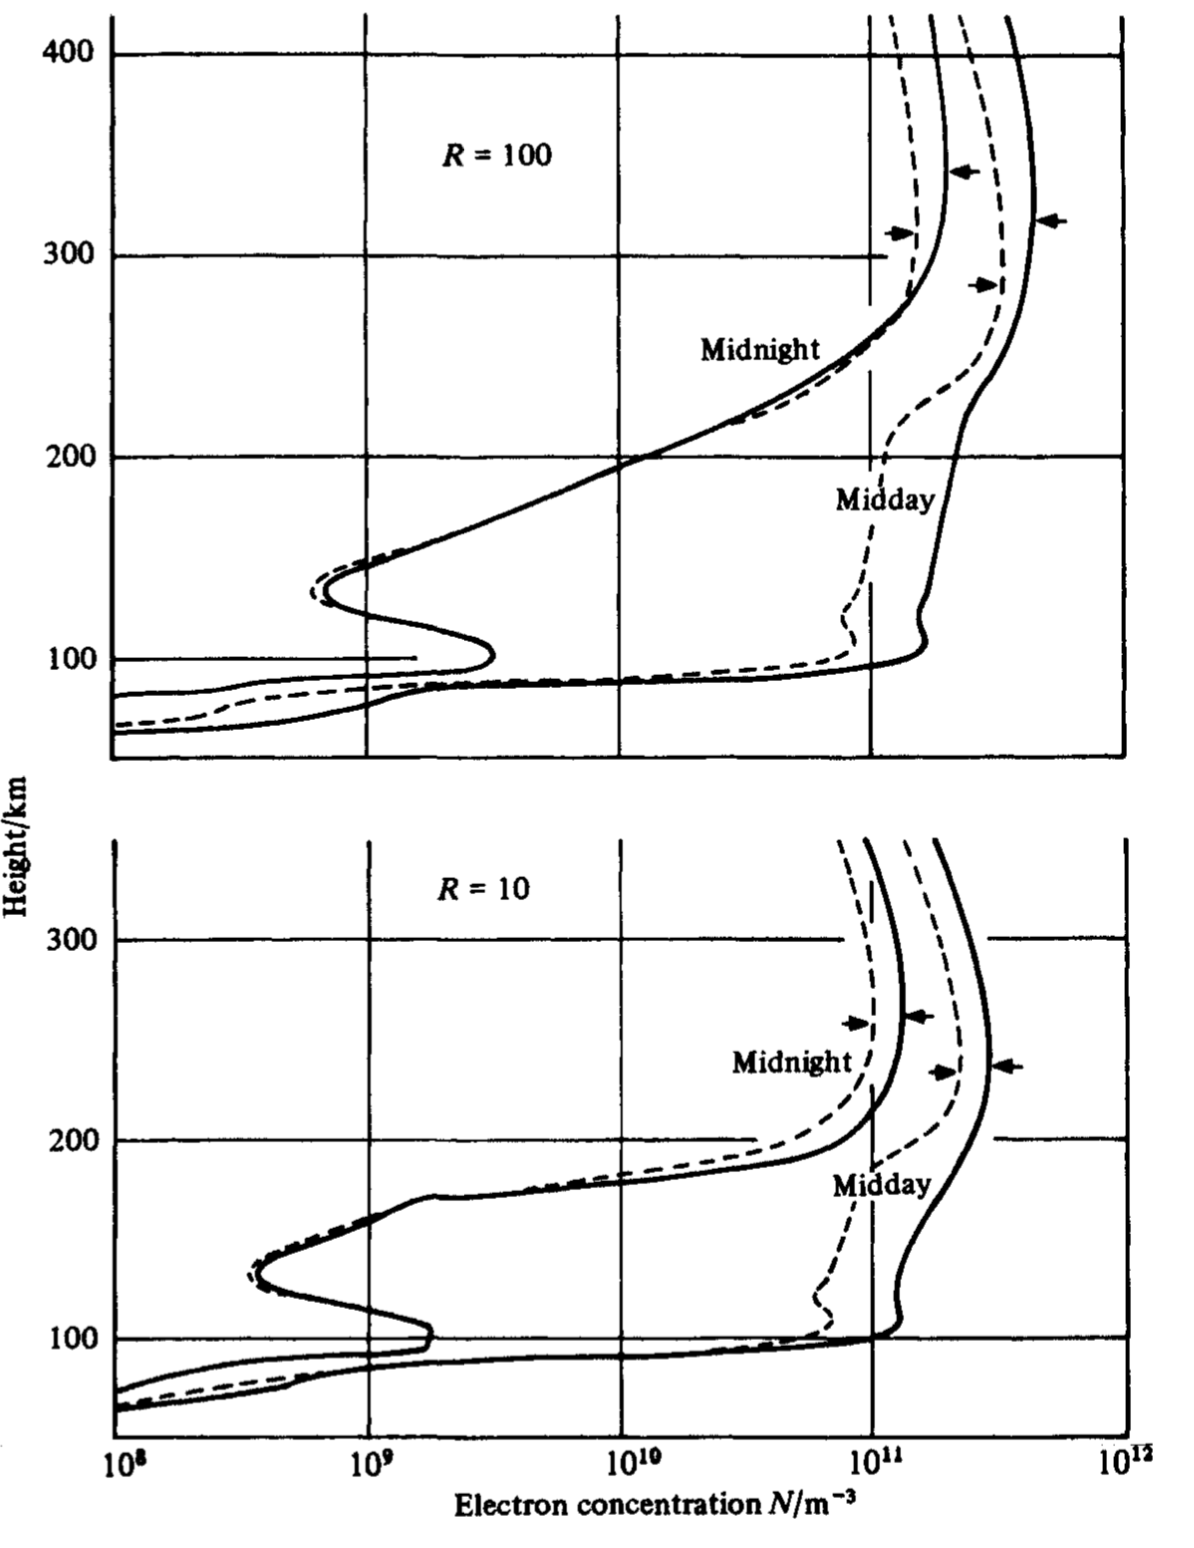
\includegraphics[width = 3in]{figs/structure_iono.png}
         \caption{}
    \label{fig:struct_ion} 
 \end{subfigure}
\qquad
 \begin{subfigure}[b]{0.44\textwidth}
         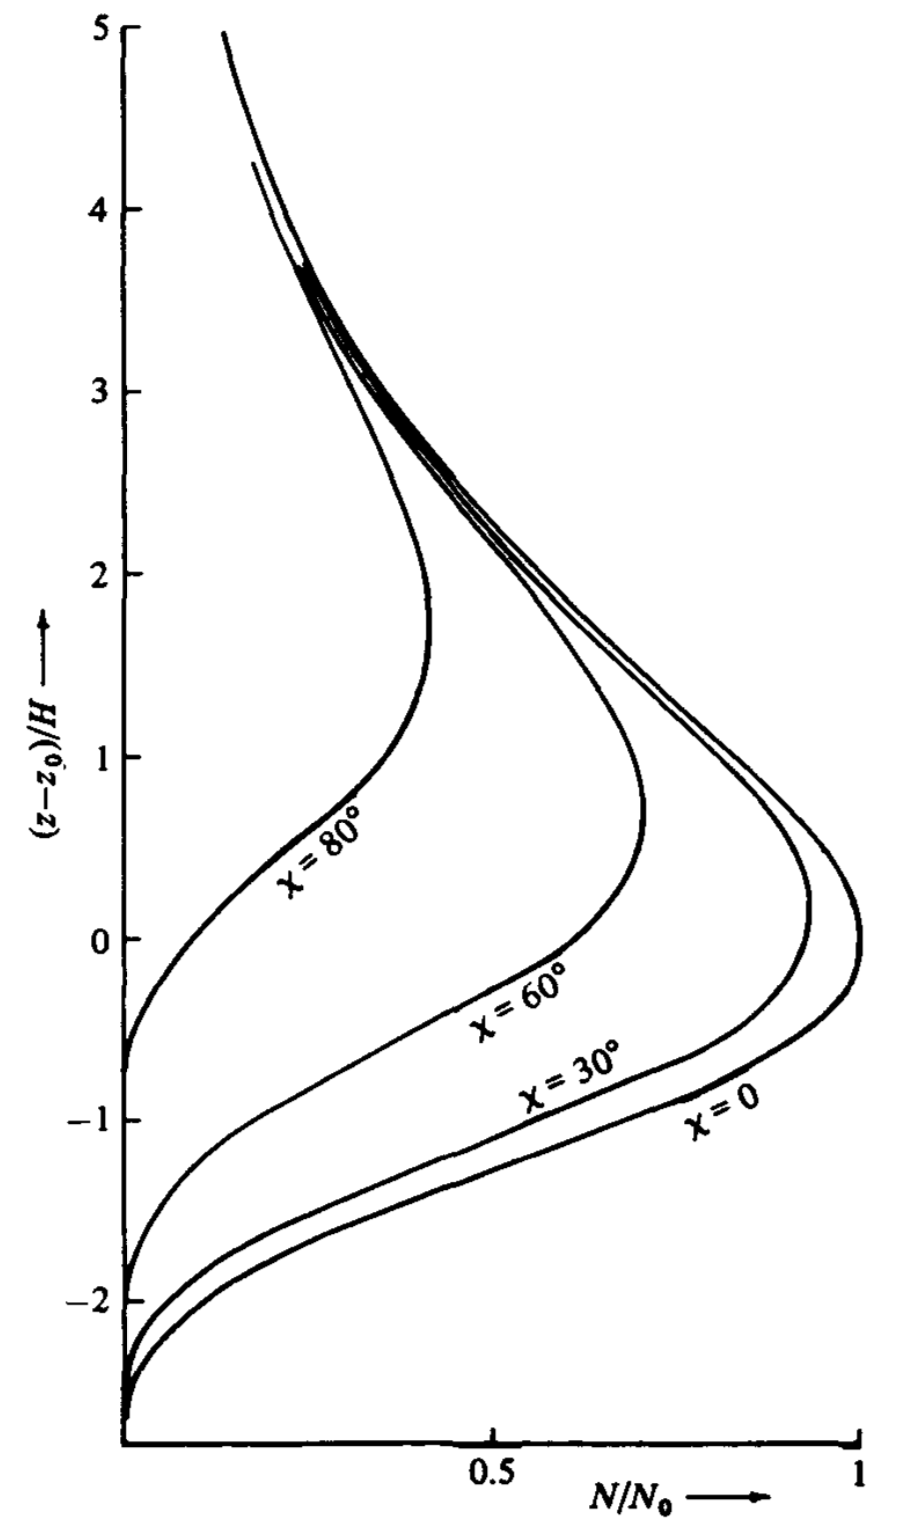
\includegraphics[width = 2.35in]{figs/chapman.png}
          \caption{ }
     \label{fig:chapman}
 \end{subfigure}
 \end{center}
 \caption{\textbf{(a)} The charge density as a function of height in the ionosphere. It also shows how the ionosphere changes at midnight and noon. Dashed lines are for January while solid lines are for June. Also given is the number of sunspots, $R$, at the time of data collection.  Figure is taken from K.G. Budden (1961).\cite{budden1988propagation} \textbf{(b)} Contour plot of the Chapman Law for various azimuthal angles of the incident sun. Figure taken from K.G. Budden (1988).\cite{budden1988propagation} }
 \label{fig:elect_density}
\end{figure}

As stated above, at a first approximation, we expect that the electron density, $N$, is only a function of the eight above the earth's surface height, $z$. More compactly, $N = N(z)$. 

    \subsubsection{Electron Density, $N(z)$} % (fold)
    \label{ssub:electron_density}
    Before we can calculate how radio-waves are reflected off of the ionosphere, we must model the ionosphere's electron density. In the early 1930's, a simple model for the electron density as a function was produced called the Chapman Law.\cite{chapman1931b,chapman1931a} 

    If we assume the Earth is constant in composition and temperature (as well as neglect the curvature of the earth\footnote{See \texttt{https://www.tfes.org/} for more information.}), then the density of the atmosphere, $\rho = \rho(z)$, is given by 
    \begin{equation}
        \rho(z) = \rho_0 e^{-M g z/ RT} = \rho_0 e^{- z/\kappa} 
        \label{eq:atm_den}
    \end{equation} where $ \kappa \equiv RT/Mg$, $\rho_0 \equiv \rho(0)$, $M$ is the average molecular weight, $g$ is the gravitational acceleration (assumed constant), $R$ is the universal gas constant,\footnote{Since all of us are ``physicists,'' we feel the need to note the definition of $R$: $R\equiv k_B N_A$ where $k_B$ is Boltzmann's constant and $N_A$ is Avogadro's number.} and $T$ is the temperature. The result of (\ref{eq:atm_den}) comes by balancing the forces acting on infinitesimal layers of atmosphere that, on a whole, is taken to be static and solving the barometric equation.\cite{schroeder1999introduction}
    
    Next, we must find the intensity of the sun that passes through the earth's atmosphere. The intensity of the sun---not surprisingly---decreases as it goes through the atmosphere.\cite{budden1961radio} Since, the sun enters at an angle from the zenith, $\alpha$. By drawing a simple diagram,\footnote{Remember, we have a flat Earth; this is a subtle but important point in this derivation.} we can see that the area normal to the incident radiation of the sun will be a factor of secant too large than the area that the ground actually receives, i.e. $dA = dA_\perp \cos\alpha.$ Since intensity is inversely proportional to $dA$, we will have the relationship of 
    \begin{equation}
        dI = I \sigma \rho \sec(\alpha) \, dz.
        \label{eq:diff_intensity}
    \end{equation}
    where $\sigma$ is a mass coefficient of absorption of the atmosphere. If we plug (\ref{eq:atm_den}) into (\ref{eq:diff_intensity}) and integrate, we get
    \begin{align}
        I(z)&= I_0 \exp\left[ -\sigma \kappa  \rho_0 \sec(\alpha) e^{- z/\kappa}\right] = I_0 \exp\left[ - \sec(\alpha) e^{- (z - z_0)/\kappa}\right]
        \label{eq:inten_v_height}
    \end{align}
    if we (cleverly) define $z_0 \equiv \kappa \ln \left(\sigma \kappa  \rho_0\right)$. The rate of absorption of energy at height $z$ is $\cos(\alpha)(dI/dz)$. If we assume that the rate of production of electrons, $q$, is proportional to this, then we get 
    \begin{equation}
        q(z) = q_0 \exp\left[1 - \frac{z-z_0}{\kappa} - \sec(\alpha) e^{- (z - z_0)/\kappa}\right].
        \label{eq:rate_prod_elec}
    \end{equation}

    Empirically---at least in the D and E-layers of the ionosphere\footnote{In the F-layer, this rate law may be equal to $dN/dt = q - b N$, but for the sake of simplicity we do not treat it as such.}---the variation of charge density is given by\cite{budden1961radio}
    \begin{equation}
        \frac{dN}{dt} = q - a N^2
        \label{eq:charge_den_rate}
    \end{equation}
    where $a$ is a ``recombination constant.'' In the steady-state solution, where $dN/dt \approx 0$, we have $N = \sqrt{q/a}$ or
    \begin{equation}
        N(z) = N_0 \exp\left[\frac12\left(1 - \frac{z-z_0}{\kappa} - \sec(\alpha) e^{- (z - z_0)/\kappa}\right)\right]
        \label{eq:chapman}
    \end{equation}
    where $N_0$ is a constant we can gather from experimental data. Quite simply, (\ref{eq:chapman}) is the Chapman Law.\cite{chapman1931a,chapman1931b,budden1961radio,budden1988propagation}


    % subsubsection electron_density (end)
    
    \subsubsection{A Modified Chapman Law, $\overline N(z,t)$} % (fold)
    \label{ssub:modified_chapman_law}
    Unfortunately, the Chapman Law is a rather simple model. It is not time dependent. It is also almost entirely qualitative due to the $\sigma$ constant that is highly dependent on what chemical species are in the atmosphere and the energy of incident light. However, it provides a good starting place to begin modifying for more accurate and simulations.

    Clearly, Fig.\ref{fig:struct_ion} demonstrates that the electron density of the ionosphere changes as a function season and time of day. In order to make the Chapman Law model of the time dependent, we can add a time dependent factor out front. To put another way, $\overline N(z,t) = T(t) N(z)$. A simple approximation is to make $T(t)$ linearly dependent on time. If we let
    \begin{equation}
        T(t) = 1 + d(t) + s(t)
        \label{eq:time_dep}
    \end{equation}
    where $d(t)$ is the ionosphere dependence on the time of day and $s(t)$ is the dependence on the season. From Fig.\ref{fig:struct_ion} we restrict the range of $d(t)$ and $s(t)$, where $d(t) \in [0,1]$ and $s(t) \in [0,4]$, respectively. These range restrictions were chosen as Fig.\ref{fig:struct_ion} demonstrates that seasonal dependence is more important than the time of day by roughly a factor of four. In our model, we input a sawtooth function for both $s(t)$ and $d(t)$ with each function's respective range. At midday, $s(t_{noon}) = 1$ and at midnight $s(t_{mid}) = 0$. Similarly, $d(t_{jun}) = 4$ while $d(t_{dec}) = 0$.

    In all, the electron-density as a function of height and time where $\overline N(t,z)$ is given by 
    \begin{align}
        \overline N(z,t) &= T(t)N(z) \nonumber \\
        &= N_0(1 + d(t) + s(t))\exp\left[\frac12\left(1 - \frac{z-z_0}{\kappa} - \sec(\alpha) e^{- (z - z_0)/\kappa}\right)\right]
        \label{eq:final_eden}
    \end{align}
    which is a simple, analytic model for the ionosphere that is used in our model.
    % subsubsection our_modified_chapman_law (end)

    \subsubsection{The Index of Refraction of the Ionosphere} % (fold)
    \label{ssub:index_of_refraction}

    To understand how to radio-waves will interact with the ionosphere, we must find an expression for the refractive index of light through the plasma. For simplicity, we are going to consider the ionosphere to be made of electrons that do not collide with one another and is isotropic throughout. When we do this, we can derive a relatively simple expression for the index of refraction of light through the medium.

    Simply put, the index of refraction relates how fast an electromagnetic wave is able to pass through a medium.\cite{jackson1999classical,townsend2000modern} We denote the index of refraction of a medium with the letter $n$; if $n = 1$ then the ray of light is moving at one of Nature's fundamental constants, $c.$

    To derive an expression for $n$ in an isotropic medium without electron collisions, we look at Maxwell's equations. In any upper-level textbook on Classical Electrodynamics, we have (from Faraday's Law of Induction)
    \begin{subequations}
           \begin{align}
       & \nabla \times \mathbf{E} = -i k \mathcal{H} \\& \nabla \times \mathcal{H} = \frac{ik}{\epsilon_0} \mathbf{D} 
    \end{align} 
    \label{eq:curls}
    \end{subequations}

    where $k$ is the wavenumber defined as $k = 2\pi/\lambda$ (where $\lambda $ is the wavelength of light), $\mathcal{H} = Z_0 \mathbf{B}$ (where $Z_0 \equiv \mu_0/\epsilon_0$ is the characteristic impedance of free space and $\mathbf{B}$ is the external magnetic field\footnote{In this case, the Earth's. Near Japan, this value is $|\mathbf{B}| \approx 47 \si{\micro\tesla}$.\cite{maus2010us}}), and $\mu_0$ and $\epsilon_0$ are the permeability and permitivity of free space, respectively.\cite{jackson1999classical,griffiths2005introduction}
    % subsubsection index_of_refraction (end)

    If we are describing a progressive plane wave,\footnote{This simply means that there is no $x$ or $y$-dependence when the waves are traveling in the $z$-direction (for Cartesian coordinates). Since we haven't chosen any coordinate system, we are free to choose any direction that $z$ points in.} we have
    \begin{align}
         \frac{\partial}{\partial x} = \frac{\partial}{\partial y} = 0, \qquad \frac{\partial}{\partial z} = -i k n
        \label{eq:plane_wave}
    \end{align}
    which when combined with equations (\ref{eq:curls}) we find
    \begin{subequations}
     \begin{align}
        \mathcal{H}_x &= - n E_y \\
        \mathcal{H}_y & = nE_x \\
        \mathcal{H}_z & = 0
    \end{align}
    \label{eq:int_step}
    \end{subequations}
    Neglecting any damping, Newton's second law can relate the electric polarization, $\mathbf{P} = Ne\mathbf{r}$ and electric field via
    \begin{align}
         &\frac{Ne}{m}\mathbf{E}e = \frac{\partial^2 \mathbf{P}}{\partial t^2}
         &\Rightarrow \mathbf{P} = -\frac{Ne^2}{m\omega^2}\mathbf{E}
         \label{eq:elec_polar}
     \end{align} 
     where we utilized the fact that the electric field varies with a phase factor, implying that $\partial^2/\partial t^2 = -\omega^2$.\cite{budden1961radio,budden1988propagation} 

     Using (\ref{eq:elec_polar}), defining $X \equiv  N e^2/\epsilon_0m \omega^2$, and enforcing our plane-wave relations of (\ref{eq:plane_wave}) we get 
     \begin{subequations}
         \begin{align}
             n \mathcal{H}_y &= E_x(1 - X) \\
            -n \mathcal{H}_x &= E_y(1 - X) \\
            0 &= E_z
         \end{align}
     \end{subequations}
     which, when utilizing equations (\ref{eq:int_step}), we can find the refractive index as
     \begin{equation}
          n^2 = 1 - X = 1 - \frac{N e^2}{\epsilon_0 m \omega^2}
      \end{equation}
      which is independent in of the direction that the radio-wave travels, but is dependent on its frequency and some fundamental constants.\footnote{So long as the radio-wave is purely a transverse wave and has no longitudinal component or the longitudinal component is negligible, this holds.}

% subsection the_ionosphere (end)

\subsection{The Ocean} % (fold)
\label{sub:the_ocean}

\subsubsection{Data Collection} % (fold)  
\label{ssub:data_collection}

To have the most accurate physical model of the ocean near Japan, we decided to take data from a weather station and fit a function to it. We took the data from one of the National Oceanic and Atmospheric Administration's (NOAA) Pacific Marine Environmental Laboratory Ocean Climate Stations. Specifically, we took data from Station Number 280401. 

Each day, the station recorded the sea surface temperature and salinity multiple times per day. The times at which they took each sample, unfortunately, were not recorded. Because of this, we assumed that the measurements were taken at regular intervals. Using this assumption, we took four averages of the temperature and salinity of the ocean corresponding to times of 2:00\,am, 8:00\,am, 2:00\,pm, and 8:00\,pm each day. 
 
It turns out that the refractive index for ratio-waves is approximately constant and the reflection coefficient is essentially one.\cite{seawater_index} So there was no temperature or salinity dependence. So that was a huge waste of time on our part.\footnote{sigh.} 


\subsubsection{Quasi-Index of Refraction of Turbulent Oceans} % (fold)
\label{ssub:ocean_ind_of_ref}
We found that ocean waves behave essentially as a mirror with an reflection coefficient of 1, so there is no appreciable index of refraction that is measured.\cite{seawater_index} However, we expect that for very turbulent waters, that the intensity of incident light will decrease as it gets scattered in various directions. Essentially, turbulent waters create a quasi-index of refraction, which we will call $m.$

\begin{figure}[ht]
 \begin{center}
     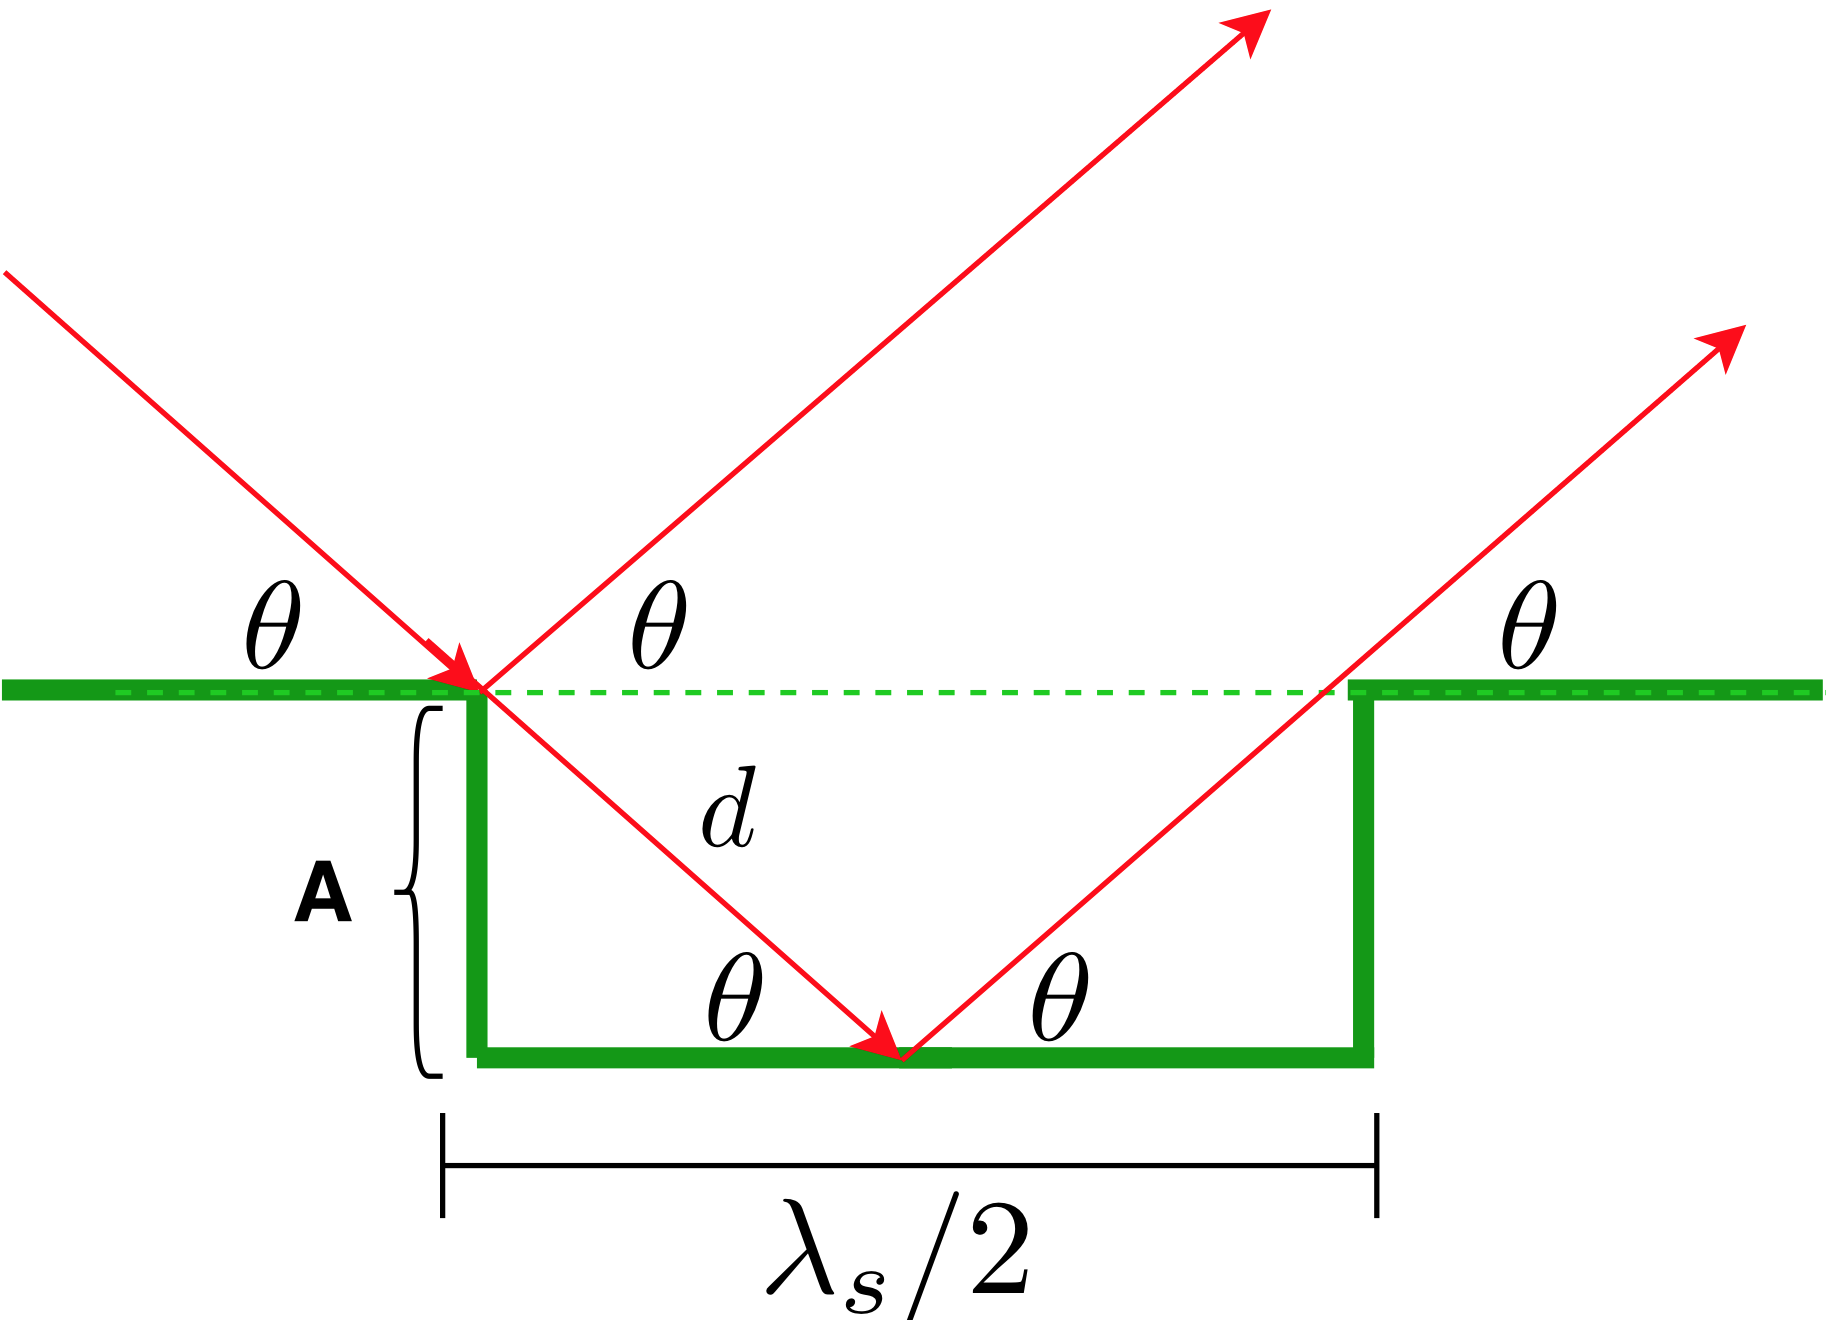
\includegraphics[width = 3.in]{figs/ocean.png}
 \end{center}
 \caption{Diagram showing our simple model of an ocean wave with an incident HF signal interacting with the ocean wave.}
 \label{fig:ocean}
\end{figure}

When a radio-wave (or any electromagnetic wave for that matter) reflect off of surface with a different index of refraction, we can find the reflection coefficient, $R$, where $R$ is defined to be the ratio of intensity of reflected light to the intensity of incident light. The relationship between $R$ and the two indices of refraction is given by a well known relation\cite{jackson1999classical,griffiths2005introduction}
\begin{equation}
    R \equiv \frac{I_r}{I_0} = \left(\frac{n-m}{n+m}\right)^2.
    \label{eq:refl_coef}
\end{equation}
where $n$ is the index of refraction of air (in our case) and $m$ is our quasi-index of refraction for turbulent water. Solving (\ref{eq:refl_coef}) for $m$ we obtain
\begin{equation}
    m = n \, \frac{1 - \sqrt R}{1+\sqrt{R}}.
    \label{eq:quasi_index}
\end{equation}


Next, we need to determine how much of $R$ we expect given ocean conditions. If we consider a simple model of ocean waves as a square wave with amplitude $A$ and a wavelength $\lambda_s$. Drawing parallel rays of light with an incident angle $\theta$, we can see that the rays of light that travel and reflect off the well of the square wave travel an extra distance of $2d$ (Fig.\ref{fig:ocean}). This leads to a phase factor where the light from one wave can interfere with another by creating a phase shift between light that hits the crest and light that hits the trough. We will define this phase shift as $\phi$ where 
\begin{equation}
    \phi = \frac{2d}{\lambda} = \frac{2}{\lambda}\sqrt{A^2 + (\lambda_s/4)^2}.
\end{equation}
The amplitude difference between the incoming and out-coming light must be proportional to the phase difference between them up to a constant. In other words, $R \propto |1+e^{i\phi}|^2 = 4 \cos^2(\phi/2)$. To find out what the constant of proportionally is between them, we consider a limiting case where we have a single incident photon. At best, we get a perfect reflection. At worst, we have the photon absorbed. Consequently, $R \in [0,1]$. Thus, we have
\begin{equation}
    R =  \cos^2\left(\frac\phi2\right).
    \label{eq:refl_coef_phi}
\end{equation}
By using (\ref{eq:refl_coef_phi}) we can calculate $m$ in (\ref{eq:quasi_index}) which is used in the time evolution of our HF signals. It is important to note, however, that taken together (\ref{eq:refl_coef_phi}) and (\ref{eq:quasi_index}) suggests that $m \le 1$. For physical refractive indices, this does not make sense. However, since we have a ``quasi-refractive index,'' we are not necessarily bound by the same conditions. Consequently, this is still meaningful in our model.

\subsubsection{Modeling Approach}
To implement the theory above, all of which underlies our model, we chose to have a stand alone radio wave model of signal propagation which is dependent on the turbulence value (a number in the range 0-1) and the indices of refraction of the ionosphere and ocean given time of day, time of year, and incident radio frequency. 

% subsubsection curve_fitting (end)

% subsubsection data_collection (end)
% subsection the_ocean (end)

% section model (end)

\subsection{Implementation in Python and Matlab}

\subsubsection{Implementation Approach}
We chose to use a suite of original scripts in Python and MATLAB to implement our model. The general architecture consists of a few main files
\begin{itemize}
\item \verb|component_params.csv|
\item \verb|constants.py|
\item \verb|input_signal.py|
\item \verb|run_radio.sh|
\item \verb|radio.py|
\item \verb|ionosphere.py|
\item \verb|ocean.py|
\item \verb|make_gif.m|
\end{itemize}

The first item a user should consider is the file \verb|component_params.csv| which contains the amplitude, angular frequency, phase shift, and offset parameters for as many Fourier components as the user would like. For our modeling, we chose to work with two Fourier components yielding the total input signal
\begin{equation}
f_{0}(t) = \sin(t) + 2\sin(0.5t)
\end{equation}
\par The \verb|constants.py| file contains all of the constants used in our model, from electrical conductivity of air to altitude of the ionosphere.
\par The file \verb|input_signal| takes the parameters of the constituent Fourier components, along with other parameters specified by the user in the Bash script \verb|run_radio.sh|, and produces a csv file with a vector of $z$ values, a vector of $t$ values, and a vector of $f_{0}(t)$ values. Recall, $f_{0}(t) = {\bf \tilde{E}}_{I}({\bf r}, t)$ which is a function of $z$ and $t$ where we have chosen the direction of propagation to be parallel to the Earth's surface and we have called that direction $z$.
\par The Bash script \verb|run_radio.sh| executes the files \verb|input_signal.py| and \verb|radio.py|. At the top of the file, users can specify the number of samples of the continuous input signal, the distance from receiver to transmitter, the time over which we observe the signal decay, the angle of incidence (defined as positive from parallel to Earth's surface), and the turbulence of the ocean.
\par The meat of the model is contained in \verb|radio.py| which calls functions contained in \verb|ionosphere.py| and \verb|ocean.py| in order to compute index of refraction as a function of each Fourier component in the frequency domain. The file first decomposes the time domain signal into its frequency components. It then modifies each component according to Fresnel's equations and the dispersion effects derived above. It then uses the inverse Fourier Transform to obtain the resulting signal when it reaches the transmitter. It outputs a \verb|.csv| file which is used for subsequent visualization.
\par To visualize what is happening to our radio wave signal as it propagates across the ocean, we use the MATLAB script \verb|make_gif.m| which not only produces a \verb|.gif| of the signal decay over the time specified in the Bash script, but also plots the initial and final signals against each other in the frequency domain and time domain.

\subsubsection{Choosing Indices of Refraction}
To consider the two cases of a turbulent sea and a calm sea, we looked at the limiting behavior of the quasi-index of refraction. For a calm sea, $A \to 0$ and $\lambda_s \to 0$ because the sea does not wave when calm. This leads to a value of $R=0$ which yields the maximum quasi-index of refraction possible: $m=1$. For a rough sea, $A$ and $\lambda_n$ are both large, but for large enough values $\phi$ will circle round and round the unit circle and average to the calm sea case. So, for the turbulent ocean case, we take $\Phi=2/\lambda$. By Taylor expansion, 
\begin{equation}
R \approx 1 - (\frac{\phi}{2})^2 = 1 - \frac{1}{\lambda^2} = \frac{2\pi^2\omega^2}{c^2 - 2\pi^{2}\omega^2}
\end{equation}
where $c$ is the speed of light and $omega$ is the angular frequency of the incident light. 
\par Unfortunately, this quasi-index of refraction and our model for the ionospheric index of refraction are where we ran into some issues. As an example, for an incident radio wave with frequency 15$MHz$, $m < 0$, which made Snell's Law (implemented in \verb|radio.py|) ``confused." For the ionosphere, the average index of refraction was often quite close to 1, which is the same index for air, and no reflection occurs when the indices of refraction are the same. So, while we learned a lot about modeling these two media, we ultimately chose to use the pseudo-value of 1.5 for both indices of refraction.

\subsubsection{Visualization}
Using $f_{0}(t) = \sin(t) + 2\sin(0.5t)$, $n_{iono} = n_{ocean}  = 1.5$, turbulence $=1$, distance to receiver $=8820 km$ (the distance from Tokyo to Los Angeles), a 30 second monitor period, and angle of incidence of 30 degrees, we produced the results included in Figures \ref{fig:freq_dom} and \ref{fig:time_dom}

 \begin{figure}[ht]
 \begin{center}
     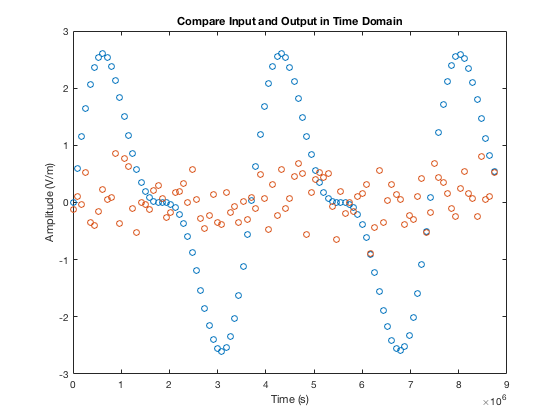
\includegraphics[width = 4.55in]{figs/time_domain_compare.png}
 \end{center}
 \caption{A comparison of the input and output signals in the time domain. Blue is the input and orange is the output. The signal has become quite noisy, as evidenced by the lack of a clear period in the plot.}
 \label{fig:time_dom} 
\end{figure}

 \begin{figure}[ht]
 \begin{center}
     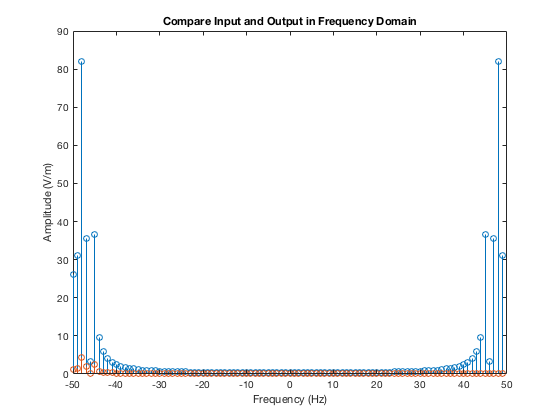
\includegraphics[width = 4.55in]{figs/freq_domain_compare.png}
 \end{center}
 \caption{A comparison of the input and output signals in the frequency domain. Blue is the input and orange is the output. The signal has become quite noisy, as evidenced by the lack of clear peaks in the stem plot.}
 \label{fig:freq_dom} 
\end{figure} 

For this set of inputs, we found that there will be 16 hops to get to the receiver. After 10 hops, the 

\section{Results} % (fold)
\label{sec:results}
 \subsection{Problem I: A Turbulent Ocean} % (fold)
 \label{sub:part_i}

 \subsection{Problem II: The Japanese Alps} % (fold)
 \label{sub:part_ii}
 West and southwest of Tokyo, Japan, there is an extensive mountain range called the Japanese Alps. This mountain range is perfect for testing how rugged, mountainous terrain affect the integrity of a signal as compared to smooth terrain or ocean.

 \subsection{Problem III: A Message to a Boat} % (fold)
 \label{sub:part_iii}
 

\section{Conclusion}
\label{sec:conclusion} 

\subsection{Analysis} % (fold)
\label{sub:analysis}


% subsection analysis (end)

\section*{Acknowledgments}
\label{sec:acknowledge}
We would like to thank our professors for lending us resources and pointing us in the direction of others. Additionally, we would also like to thank the beautiful community of StackExchange for teaching us everything we could ever need to know when we have questions we can't solve ourselves. 

 We would like to thank our College for financial support allowing us to enter this competition. Without it, we would not have been able to have this much fun or sleep deprived. \shrug\cite{townsend2000modern} 

\newpage
\section*{Appendix: Constants Used in Code}
\lstinputlisting[language=Python]{../model/constants.py}
%%%%%%%%%%%%%%%%%%%%%%%%%%%%%%%%%%%%%%%%%%%%%%%%%%%%%%%%%%%%%%%%%%%%%%%
%% Bibliography
%%%%%%%%%%%%%%%%%%%%%%%%%%%%%%%%%%%%%%%%%%%%%%%%%%%%%%%%%%%%%%%%%%%%%%%
\newpage 
% \nocite{*}
\bibliographystyle{plainnat}
\bibliography{solution}

\end{document}
